% === Begin Label Data ===
% ID: 760
% 难度星级: 
% 标签: 
% 备注: 
% 组卷引用次数: 0
% === End  Label Data ===

\begin{problem}{2025}{G}{上海春季卷}{12}{向量}
在平面中，$\vec{e}_1$ 和 $\vec{e}_2$ 是互相垂直的单位向量，向量 $\vec{a}$ 满足 $|\vec{a}-4\vec{e}_1|=2$，向量 $\vec{b}$ 满足 $|\vec{b}-6\vec{e}_2|=1$，则 $\vec{b}$ 在 $\vec{a}$ 方向上的数量投影的最大值为\underline{\hspace{4em}}.
\end{problem}

\begin{answer}
$4$
\end{answer}

\begin{solutions}
 如图建立平面直角坐标系，其中 $\vec{e}_1=(1,0)$，$\vec{e}_2=(0,1)$.设 $\vec{a}=\overrightarrow{OA}$，$\vec{b}=\overrightarrow{OB}$，则 $A$ 在圆 $C_1:(x-4)^2+y^2=4$ 上运动，$B$ 在圆 $C_2:x^2+(y-6)^2=1$ 上运动。

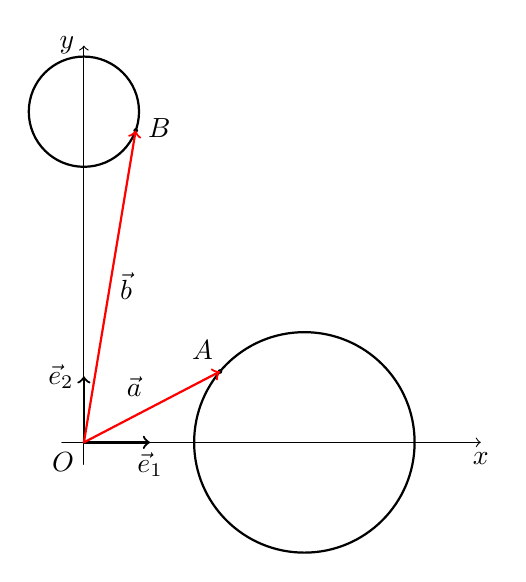
\begin{tikzpicture}[line cap=round,line join=round,scale=0.7]
\usetikzlibrary{calc}

% ---- axes (with dashed inner guides like the picture) ----
\draw[->] (-0.4,0) -- (7.2,0) node[below] {$x$};
\draw[->] (0,-0.4) -- (0,7.2) node[left] {$y$};
\node[below left] at (0,0) {$O$};

% unit vectors e1,e2
\draw[->,thick] (0,0) -- (1.2,0) node[below] {$\vec e_1$};
\draw[->,thick] (0,0) -- (0,1.2) node[left] {$\vec e_2$};

% ---- circles: C1 centered at (4,0) radius 2; C2 centered at (0,6) radius 1 ----
\draw[thick] (4,0) circle (2);
\draw[thick] (0,6) circle (1);


% ---- points A on C1 and B on C2 (choose a representative placement) ----
\coordinate (A) at ($(4,0)+(140:2)$);
\coordinate (B) at ($(0,6)+(-20:1)$);

\fill (A) circle (1.2pt);
\node[above left] at ($(A)+(0.05,0.05)$) {$A$};

\fill (B) circle (1.2pt);
\node[right] at ($(B)+(0.05,0.05)$) {$B$};

% ---- vectors a=OA and b=OB (red) ----
\draw[red,thick,->] (0,0) -- (A) node[midway,above left,black] {$\vec a$};
\draw[red,thick,->] (0,0) -- (B) node[midway,right,black] {$\vec b$};

\end{tikzpicture}

$\vec{b}$ 在 $\vec{a}$ 方向上的数量投影是 $f(\vec{a},\vec{b})=|\vec{b}|\cos\langle\vec{a},\vec{b}\rangle=\dfrac{\vec{a}\cdot\vec{b}}{|\vec{a}|}$.

思路 1：设 $\theta=\langle\vec{a},\vec{b}\rangle$（$\theta$ 是 $\vec{a}$，$\vec{b}$ 的函数）。为求 $\max\limits_{\vec{b}}\max\limits_{\vec{a}}f(\vec{a},\vec{b})$，先固定点 $B$，研究 $\max\limits_{\vec{a}}f(\vec{a},\vec{b})$ 即 $\max\limits_{\vec{a}}\{|\vec{b}|\cos\theta\}$.而当 $B$ 固定时，$|\vec{b}|$ 是定值，所以 $|\vec{b}|\cos\theta$ 的最大值只和 $\theta$ 有关。

对任意固定的点 $B$，当 $OA$ 与圆 $C_1$ 相切且 $A$ 位于第一象限时，$\theta$ 达到最小值。此时 $\vec{a}=(3,\sqrt{3})$.

因为 $B$ 在圆 $C_2$ 上，取 $\vec{b}=(\cos\beta,6+\sin\beta)$，则
$$
f(\vec{a},\vec{b})=\dfrac{\vec{a}\cdot\vec{b}}{|\vec{a}|}=\dfrac{3\cos\beta+\sqrt{3}\sin\beta+6\sqrt{3}}{2\sqrt{3}}=\dfrac{2\sqrt{3}\left(\dfrac{\sqrt{3}}{2}\cos\beta+\dfrac{1}{2}\sin\beta\right)+6\sqrt{3}}{2\sqrt{3}}=\cos\left(\beta-\dfrac{\pi}{3}\right)+3.
$$

所以，当 $\beta=\dfrac{\pi}{3}$，即 $B\left(\dfrac{1}{2},6+\dfrac{\sqrt{3}}{2}\right)$ 时，$\vec{b}$ 在 $\vec{a}$ 方向上的数量投影取得最大值 $4$.

思路 2：设 $\vec{a}=(4+2\cos\alpha,2\sin\alpha)$，$\vec{b}=(\cos\beta,6+\sin\beta)$.

则 $\vec{b}$ 在 $\vec{a}$ 方向上的数量投影为
$$
f(\vec{a},\vec{b})=\dfrac{\vec{a}\cdot\vec{b}}{|\vec{a}|}=\dfrac{(4+2\cos\alpha)\cos\beta+2\sin\alpha(6+\sin\beta)}{\sqrt{(4+2\cos\alpha)^2+(2\sin\alpha)^2}}
$$
$$
=\dfrac{12\sin\alpha+(4+2\cos\alpha)\cos\beta+2\sin\alpha\sin\beta}{\sqrt{(4+2\cos\alpha)^2+(2\sin\alpha)^2}}
$$
$$
\leqslant\dfrac{12\sin\alpha+\sqrt{(4+2\cos\alpha)^2+(2\sin\alpha)^2}}{\sqrt{(4+2\cos\alpha)^2+(2\sin\alpha)^2}}=\dfrac{6\sin\alpha}{\sqrt{5+4\cos\alpha}}+1.
$$

等号成立条件是 $\tan\beta=\dfrac{4+2\cos\alpha}{2\sin\alpha}$ 且 $\cos\beta\geqslant0$.

令 $t=5+4\cos\alpha\in[1,9]$，则 $\sin\alpha=\dfrac{\sqrt{-t^2+10t-9}}{4}$（$\sin\alpha<0$ 时一定不会取到最大值），

所以 $f(\vec{a},\vec{b})=\dfrac{\vec{a}\cdot\vec{b}}{|\vec{a}|}=\dfrac{3\sqrt{-t^2+10t-9}}{2\sqrt{t}}+1=1+\dfrac{3}{2}\sqrt{-t+10-\dfrac{9}{t}}\leqslant4$，

等号成立条件是 $t=3$，此时 $\cos\alpha=-\dfrac{1}{2}$，$\sin\alpha=\dfrac{\sqrt{3}}{2}$，$\tan\beta=\sqrt{3}$，$\beta=60^\circ$.于是，当 $\vec{a}=(3,\sqrt{3})$，$\vec{b}=\left(\dfrac{1}{2},6+\dfrac{\sqrt{3}}{2}\right)$ 时，$\vec{b}$ 在 $\vec{a}$ 方向上的数量投影 $\dfrac{\vec{a}\cdot\vec{b}}{|\vec{a}|}$ 取得最大值 $4$.
\end{solutions}